\setcounter{part}{23}  % O

\part{Optique}
\section{Optique géométrique}
\begin{exercise}{Cascade de Yelowstone}{2}{Sup}
{Optique,Optique géométrique}{lelay,bermudez}

\begin{figure}[H]
    \centering
    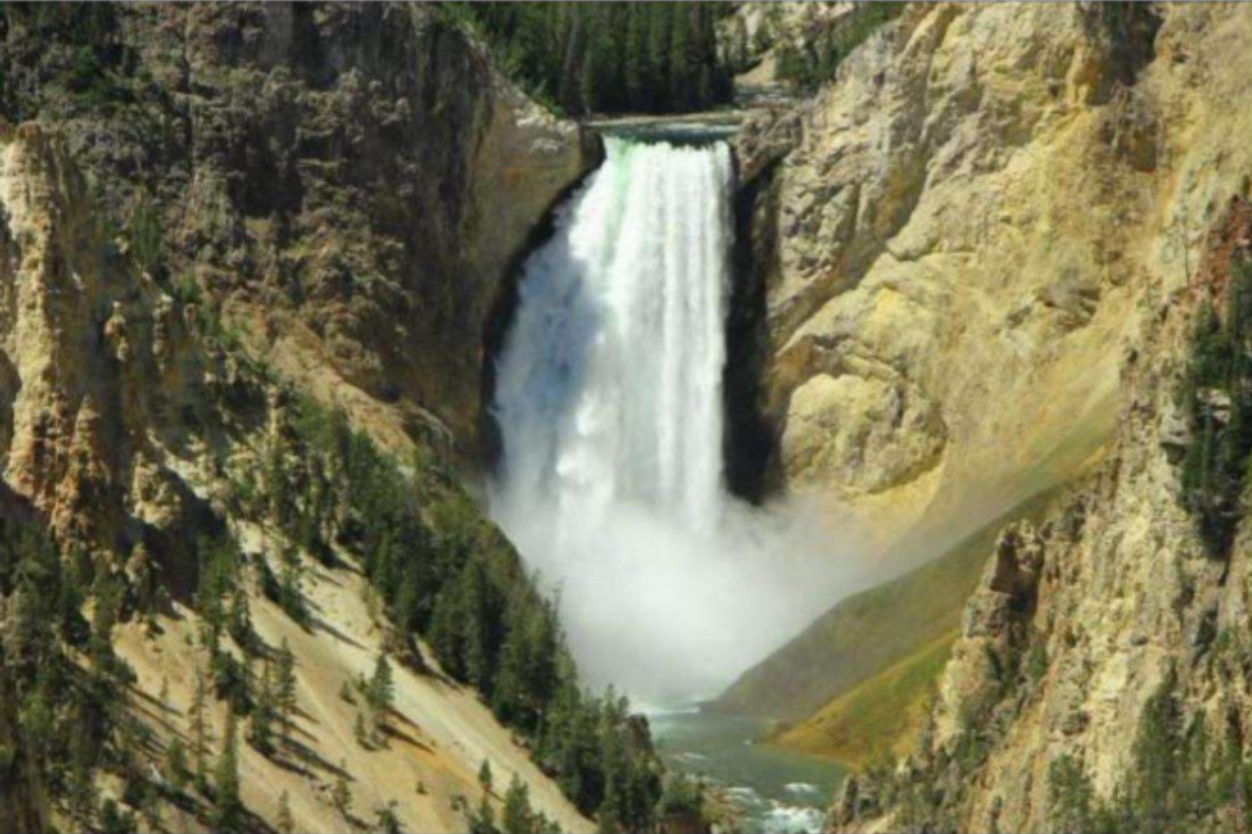
\includegraphics[width=1.\linewidth]{optique/optiquegeometrique/cascade1.png}
    \caption{Photographie de la cascade inférieure de Yellowstone vue de Red Rock Point. \newline (Nikon F, pellicule Kodak Kodachrome 35 format $24\times 36$ mm, téléobjectif $f'= 90$ mm).}
\end{figure}

\begin{figure}[H]
    \centering
    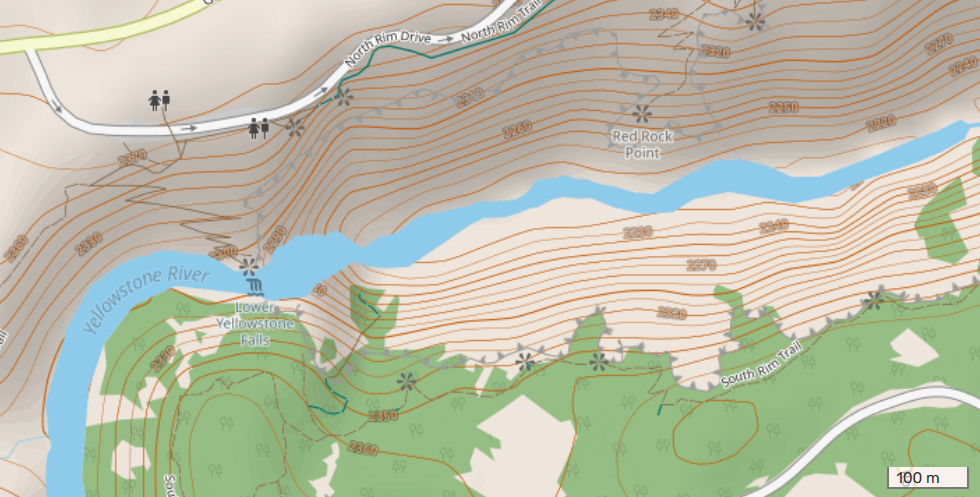
\includegraphics[width=1.\linewidth]{optique/optiquegeometrique/cascade2.png}
    \caption{Carte topographique du Canyon de Yellowstone, avec la cascade inférieure et Red Rock Point.}
\end{figure}

\textsfbf{Problème ouvert :} À l’aide des documents et de vos connaissances, estimer la hauteur de la cascade inférieure de la rivière Yellowstone dans le Grand Canyon (Wyoming, États-Unis). \newline
Valider cet ordre de grandeur en vous aidant des lignes de niveau sur la carte topographique.

\end{exercise}

\begin{solution}
    Relation de conjugaison sur le grandissement :
    $$\gamma = \dfrac{\bar{A'B'}}{\bar{AB}} = -\frac{f'}{\bar{FA}}.$$
    On obtient avec les documents :
    \begin{itemize}
        \item $\bar{A'B'} = -17$ mm
        \item $\bar{FA} \simeq D = \text{distance photographe--cascade} = 245$ m.
        \item $f' = 90$ mm
    \end{itemize}
    D'où $H = \bar{AB} = D\dfrac{-\bar{A'B'}}{f'} = 94$ m.

    On compte bien environ 9 lignes de niveau entre le haut et le bas de la cascade.
\end{solution}
\begin{exercise}{Photo aillée}{2}{Sup}
{Interference, Michelson}{lelay, centrale}

Une tête d'ail fait à peu près 7 cm de diamètre. Cette photo a été prise à une distance $D$ de l'ail avec un appareil de distance focale $f' = 50$ mm en utilisant un diaphragme de rayon $R$ et une pellicule de 24x36 mm placée à une distance $d$ de la lentille.

\begin{figure}[H]
    \centering
    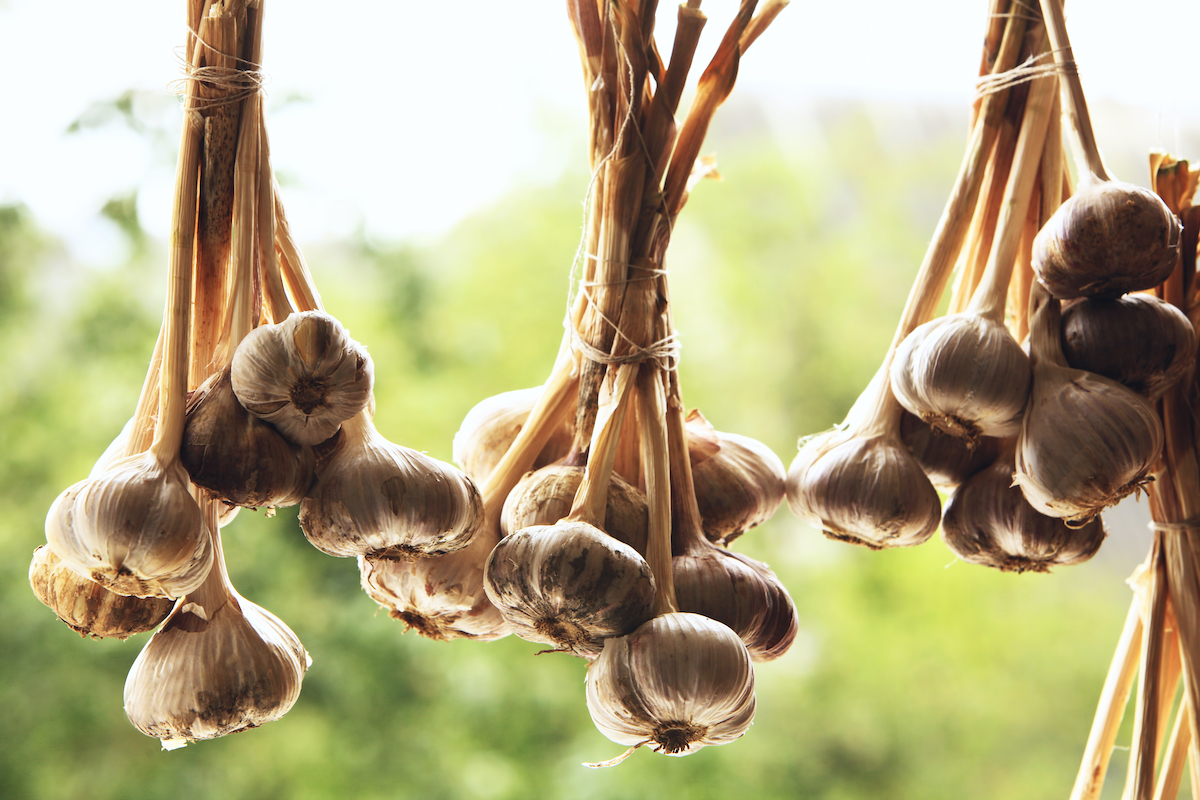
\includegraphics[width=.8\linewidth]{optique/optiquegeometrique/ail.jpg}
    \caption{Ail.}
\end{figure}

\begin{questions}
    \questioncours Lentilles convergentes, relations de conjugaisons.
    \question Déterminer la taille des gousses d’ail sur la pellicule. En déduire $d$ et $D$.
    \question On voit sur la photos des ronds clairs qui viennent d’objets au loin. Déterminer leur taille sur la pellicule, en déduire le rayon
du diaphragme $R$. Donner le nombre d'ouverture de l'appareil $\frac{f'}{2R}$.
    \question À quel phénomène aurait-on pu penser pour expliquer ronds ? Montrer quantitativement que ce n’est pas dû à cette cause.
    \question Quelle semble être la distance maximale jusqu’à laquelle on voit net ? En déduire la taille d’un élément photosensible sur cette
pellicule. Comparer à la résolution en pixels d’un appareil récent.
\end{questions}

\end{exercise}

\begin{solution}
\begin{questions}
    \questioncours $1/D+1/d=1/f'$ (Descartes)
    \question Avec un schéma et Thalès on trouve que $\frac{d}{D} ={5\text{ mm}}{7\text{ cm}}$ soit $D=75$ cm et $d=54$ mm.
    \question On prend un rayon qui vient de l’infini, si on appelle $\delta$ la taille d'un rond sur la pellicule ($\sim 1.7$ mm) alors par Thalès $\frac{\delta/2}{R}=\frac{d-f'}{f'}$ on trouve $R$ de l'ordre de $1$ cm.
    \question La diffraction. OdG de diffraction, on a $\lambda \ll R$ donc c'est mort.
    \question On voit net sur a peu pres 1 tête soit une profondeur de champ d'une dizaine de cm. Un objet situé à $D-5$ cm serait nette dans le plan situé à $d+\delta d = 57$ mm. Thalès ensuite avec les deux plus grands rayons venant de cet objet sur l'axe optique donne $\frac{\epsilon}{R} = \frac{\delta d}{d+\delta d}$ soit ici a peu près 0.5 mm. On trouve un elment photosensible de 0.1 mm$^2$ ce qui est grand devant la taille en pixel des caméras récentes.
\end{questions}
\end{solution}
\begin{exercise}{Le pont}{2}{Sup}
{Optique}{lelay}

La photographie du pont ci-dessous (hauteur spécifiée sur le panneau : 4,30 m) a été réalisée avec un appareil photo 
argentique :
\begin{itemize}
    \item Format de l’image sur la pellicule : 24 mm x 36mm
    \item Distance focale de l’objectif assimilé à une lentille mince convergente de focale : $f’$ = 35 mm
\end{itemize}

\begin{figure}[H]
    \centering
    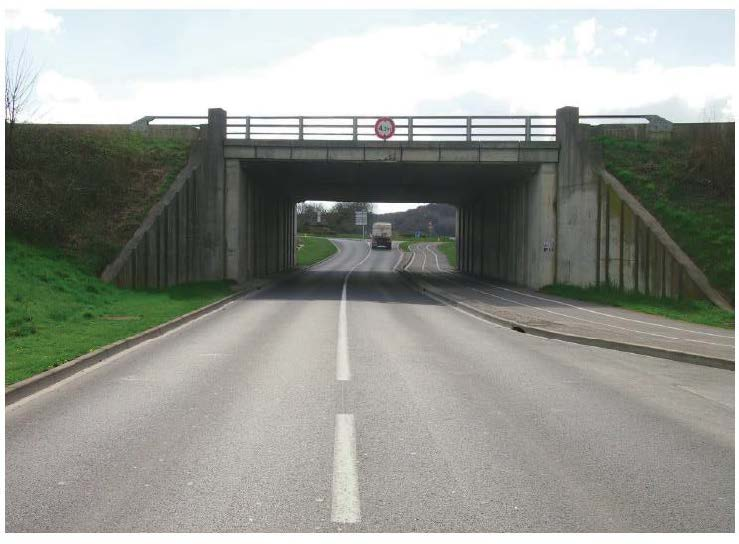
\includegraphics[width=1.\linewidth]{optique/optiquegeometrique/POOOOOOONT.jpg}
    \caption{Pont.}
\end{figure}

\begin{questions}
    \questioncours Foyers optiques, distance optique, vergence.
    \question Estimer la profondeur $p$ du pont et la distance $D$ entre l'entrée du pont et l'appareil photographique.
\end{questions}

\end{exercise}

\section{Lois de la réfraction}
\begin{exercise}{Arc en ciel}{3}{Sup}
{Réfraction, Optique géométrique}{bermudez}

Un arc-en-ciel se forme lorsqu'un observateur voit par réflection un rideau de gouttes d'eau.

On considère un rayon lumineux qui entre en E sous incidence $i$ dans une goutte d'eau sphérique de rayon $R$ et d'indice optique $n_\text{e}$. Après plusieurs réflections--réfractions, il ressort de la goutte au point S en ayant dévié d'un angle $D$.

La loi de Cauchy établi la relation entre l'indice optique d'un milieu $n$ et la longeur d'onde :
$$n(\lambda) = A + \dfrac{B}{\lambda^2}.$$

\begin{figure}[H]
\centering
\begin{tabular}{rr|ll}
    Milieu & & $A$ & $B$ (nm$^2$)  \\ \hline
    Verre (BK6) & $n_\text{v}$ & $1,5$ & $4\times 10^{3}$ \\
    Eau & $n_\text{e}$ & $1,3$ & $5\times 10^{3}$ \\
    Air & $n_\text{a}$ & $1,0$ & $\sim 0$ \\ \hline
\end{tabular}

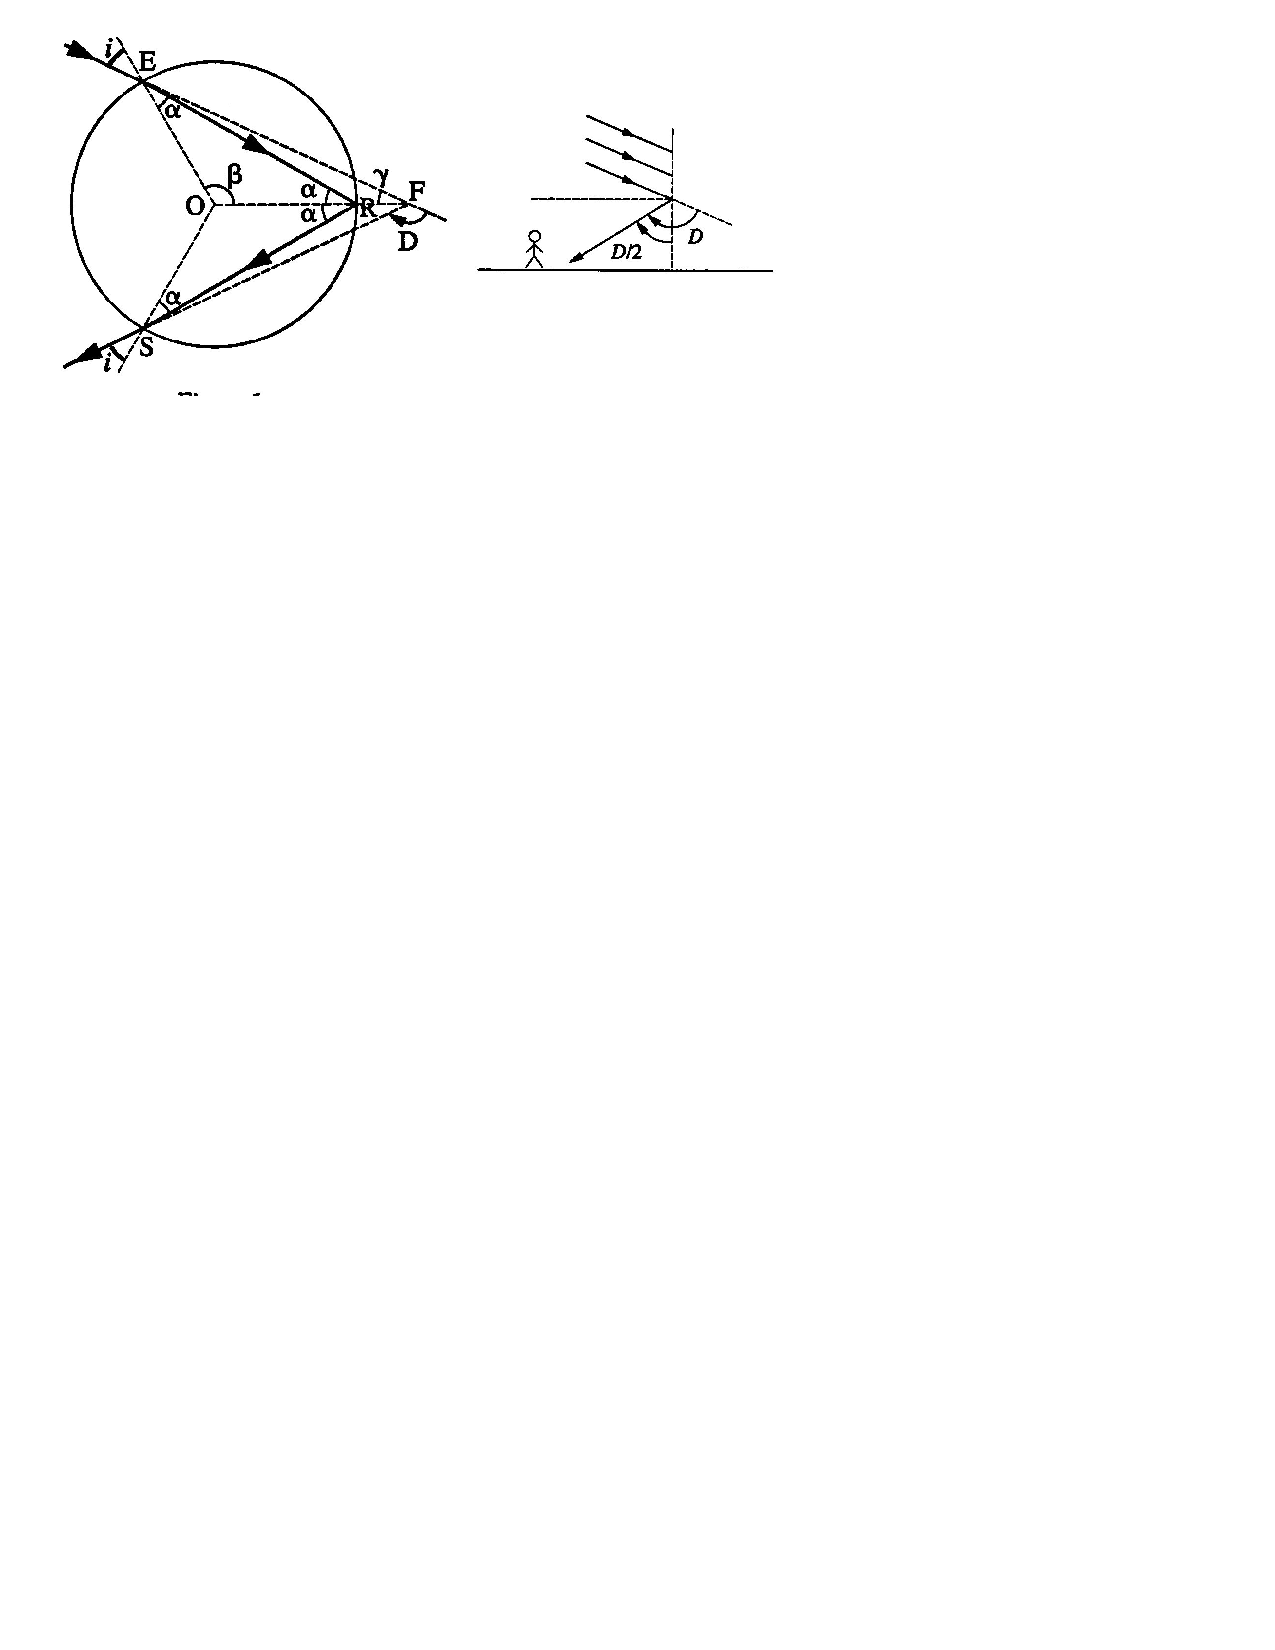
\includegraphics[width=\linewidth]{optique/refraction/arc-en-ciel.pdf}
\end{figure}

\begin{questions}
    \questioncours A l'aide de la loi de Cauchy, expliquer la décomposition de la lumière par un prisme de Newton.
    \question Déterminer l'expression de la déviation $D$ en fonction de l'angle d'incidence $i$ et de l'indice optique de l'eau $n_\text{e}$. \\ On pourra s'aider des angles $\beta$ et $\gamma$ et de leur relations dans les triangles OEF et OER. Et trouver par une autre méthode le lien entre $\alpha$, $i$.
    
    \question Calculer les déviations de part et d'autre du spectre de la lumière visible. On admettra que l'intensité lumineuse maximale est observée pour une incidence de $i = 60^\circ$ (déviation minimale). 
    
    \uplevel{Lorsqu'un rideau de pluie est éclairé par le soleil, un observateur peut voir toutes les couleurs de l'arc-en-ciel. Ce ne sont donc pas les mêmes gouttes qui produisent toutes les couleurs.
    
    Ici l'observateur à $H = 1,00$ km du rideau de pluie.}
    
    \question À quelles altitudes sont situées les gouttes qui produisent chaque extrema de l'arc-en-ciel ?  Que se passe-t-il lorsque l'observateur se rapproche de l'arc-en-ciel ? \\
    On négligera la taille de l'observateur devant l'altitude des gouttes considérées. 
\end{questions}

\end{exercise}

\begin{exercise}{Fibre$\cdot$s optique$\cdot$s}{2}{Sup}
{Réfraction, Optique géométrique}{bermudez}

On étudie la propagation d'un faisceau lumineux d'incidence $i$ dans une fibre optique formée d’une âme d’indice $n_\text{a} = 1,66$ et de rayon $r = 1$ mm entourée d’une gaine en verre d’indice $n_\text{g} = 1,52$.

\begin{figure}[H]
\centering
    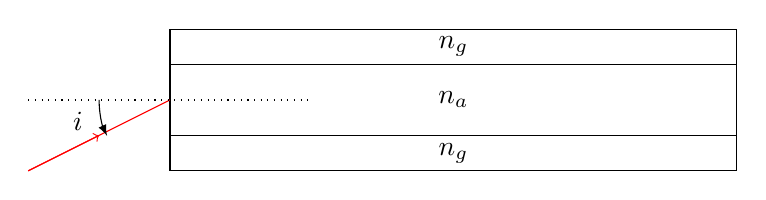
\begin{tikzpicture}[scale=.9] 
%fibre optique 
\draw (0,0) --+ (8,0); 
\draw (0,-0.5) --+ (8,0); 
\draw (0,-1.5) --+ (8,0); 
\draw (0,-2) --+ (8,0); 
\draw (0,0) --+ (0,-2); 
\draw (8,0) --+ (0,-2); 
%\draw [->,color=red] (0,-1) --++ (2,0.5) --++ (4,-1) --++ (4,1) --++ (4,-1) --++ (1,0.25); 
\draw [color=red] (0,-1) --++ (-2,-1); 
\draw [->,color=red] (-2,-2) --++ (1,0.5); 
\node at (4,-0.25) {$n_\text{g}$}; 
\node at (4,-1.75) {$n_\text{g}$}; 
\node at (4,-1) {$n_\text{a}$}; 
\draw [dotted](-2,-1)--++(4,0); 
\draw [->,>=latex] (-1,-1) arc (0:25:-1.2); 
\node () at (-1.3,-1.3) {$i$}; 
\end{tikzpicture}
\end{figure}

\begin{questions}
    \questioncours Démontrer la relation de Snell--Descartes à partir du principe de Fermat.
    \question \textsf{Culture sciences--physiques :} Applications de la fibre optique. Avantages et incovéniants.
    \question Quelle l'incidence maximale $i_\text{max}$ sous laquelle le rayon est entièrement réfléchi ? On exprimera l'ouverture numérique de la fibre $\text{ON} \equiv \sin i$ en fonction des indices de la fibre.
    \question On veut se servir d'une telle fibre, sans la gaine, pour détecter la présence d'eau ($n_\text{e} = 1,33$) ou d'air (considéré comme du vide d'indice 1) dans un réservoir.
    Proposer une valeur de l'incidence pour mettre en place ce dispositif.
    
    \question Évaluer le retard $\tau$ entre l'entrée et la sortie de $L = 1$ km de fibre sous incidence $i = 8^\circ$.
    \question Une fibre réelle atténue le signal à cause de l'absorption et de la diffusion de la lumière par le matériau. Pour $\lambda = 800$ nm, on a
    $$A = 10\log(I_\text{in}/I_\text{out}) = 1,2 \mathrm{ dB\cdot km^{-1}}.$$
    Au bout de combien de kilomètres restera-t-il 10\% du flux incident ?
    
    \question On suppose l'incidence nulle, mais que la fibre est courbée avec un rayon de courbure $R = 10$ cm. Calculer l'incidence $i'$ du rayon arrivant à l'interface gaine--âme et donner une condition sur $r$ et $R$ pour que le rayon soit totalement réfléchi.
\end{questions}

\end{exercise}

\begin{exercise}{Mirages mirages}{2}{Sup}
{Réfraction, Optique géométrique}{bermudez}

\begin{questions}
    \question \textsf{Brève :} On considère un aquarium constitué d'une paroi de verre, d'indice $n_\text{v} = 1,5$ et d'épaisseur $e = 5$ mm, séparant l'air (considéré comme du vide d'indice 1) et l'eau de l'aquarium ($n_\text{e} = 1,33$). \\
    Donner le lien entre l'angle d'incidence côté aquarium et l'angle transmis coté air. Voit-on tout ce qui se passe dans l'aquarium ?
    
    \uplevel{On s'intéresse maintenant à un type de mirage similaire lié aux différences de température. L'indice de l'air $n$ est lié à la température $T$ par la loi de Gladstone qui s'énnonce comme suit :
    $$n-1 = K/T,$$ avec $K = 82$ mK.}
    
    \question \textsf{Culture sciences--physiques :} Expliquer le phénomène de mirage.
    \question On suppose que la température près du sol $T_\text{s}$ (entre $z=0$ et $z=h$) est plus élevée que la température de l'air $T_\text{a}$ ($z>h$). Pour un observateur dont les yeux sont à une hauteur $H > h$ au dessus du sol, déterminer à quelle distance minimale se situe le mirage.
\end{questions}

\end{exercise}


\section{Division du front d'onde}
\begin{exercise}{Miroirs de Lloyd}{2}{Spé}
{Interference, Michelson}{lelay}

On considère un miroir horizontal plan $M$. Un écran est placé orthogonalement à $M$, et une source lumineuse ponctuelle et monochromatique $S$ est placée à un distance $D$ de l'écran et à une distance $\frac{a}2$ du miroir.

\begin{questions}
    \questioncours Différence de marche, interférences (on illustrera avec un exemple du cours)
    \question Faire un schéma
    \question Les interférences sont obtenues par superposition sur l'écran de la lumière issue de $S$ et de la lumière réfléchie par le miroir. Quelles sont les deux sources dont sont issues les interférences ?
    \question Ces sources sont-elles cohérentes ? On rappelle que la réflexion d'une onde électromagnétique sur un miroir s'accompagne d'un déphasage de $\pi$ (est-ce un retard ou une avance de phase ?).
    \question Donner l'éclairement résultant sur l'écran. Quels points communs, quelles différences avec une expérience de trous d'Young ?
    \question Peut-on remplacer la source ponctuelle $S$ par une fente lumineuse allongée dans la direction commune au miroir et au plan sans dégrader la visibilité des franges ?
    \question (Difficile) Que se passe-t-il si on rajoute un second miroir à distance $a$ du premier, de telle sorte que la source se trouve au milieu des deux miroirs ? On répondra d'abord de manière qualitative, en faisant un parallèle judicieux avec le cours.
\end{questions}

\end{exercise} 
\begin{exercise}{Frange achromatique}{2}{Spé}
{Interference, Young}{lelay}

On considère deux fentes d'Young situés à distance $D$ d'un écran, éclairés par une source ponctuelle $S$ monochromatique de longueur d'onde $\lambda_0$ située dans le plan focal objet d'une lentille convergente.

\begin{questions}
    \questioncours Fentes d'Young. Décrire la figure d'interférence observée ainsi que la répartition de l'éclairement $\cal{E}(x)$ sur l'écran.
    \uplevel{Une lame de verre, d'épaisseur $e$ et d'indice $n$ est placée devant une des fentes.}
    \question Déterminer l'expression de l'éclairement sur l'écran dans cette nouvelle situation. Quelle est la nouvelle position de la frange centrale ? De combien d'interfranges s'est-elle déplacée ?
    \uplevel{On remplace désormais la source monochromatique par une source de lumière blanche. L'indice du verre varie avec la longueur d'onde dans le vide selon la loi de Cauchy : 
    $$ n(\lambda) = A + \frac{B}{\lambda^2}$$
    avec $A = 1.489$ et $B = 0.004$ $\mu$m$^2$. On appelle \textit{frange achromatique} celle pour laquelle $\pdv{\Delta\varphi}{\lambda} = 0$ pour $\lambda = \lambda_m = 600$ nm la longueur d'onde moyenne du spectre visible.}
    \question Déterminer la position de la frange achromatique. Donner, en interfrange, l'écart entre la frange achromatique et la frange centrale trouvée à la question précédente.
    \question On veut mesurer l'épaisseur $e$ de la lame en trouvant le déplacement de l'unique frange blanche (qui est la mieux contrastée) dû à l'ajout de la lame. Quelle erreur relative comment-on sur la mesure de $e$ si on considère $n = 1.500$, indépendamment de la longueur d'onde ?
\end{questions}

\end{exercise}
\begin{exercise}{Source étendue}{3}{Spé}
{Interference, Young}{bermudez,lelay}

On considère deux trous d'Young situés à distance $D$ d'un écran, éclairés par une source ponctuelle $S$ monochromatique de longueur d'onde $\lambda_0$ située dans le plan médian des trous à une distance $L$ de leur point milieu.

\begin{questions}
    \questioncours Trous d'Young. Décrire la figure d'interférence observée ainsi que la répartition de l'éclairement $E(x)$ sur l'écran.
    \uplevel{On remplace la source $S$ (de puissance $P_0$) par deux sources incohérentes $S_1$ et $S_2$ (chacune de puissance $P_0/2$) situées à une distance $\pm \frac{b}{2}$ de $S$ dans la direction verticale.}
    \question Déterminer l'expression de l'éclairement sur l'écran dans cette nouvelle situation. On mettra en valeur un terme nouveau, la visibilité $V$. Comment faut-il choisir $b$ pour avoir la figure d'interférence la plus nette possible (i.e. la meilleure visibilité ?
    \question On considère le cas d'une source étendue de puissance $P_0$ de taille $B$. Expliquer pourquoi il est équivalent de considérer un continuum de couples de sources infinitésimales incohérentes écartées de $b$, de puissance $\dd{P} = P_0 \frac{\dd{b}}{2B}$ avec $b$ variant entre $0$ et $B$.
    \question Quel est l'éclairement total de l'écran dans ce cas ? Comment choisir $B$ pour conserver la figure d'interférence la plus nette possible ?
    \question En réalité, il est impossible d'obtenir une source purement ponctuelle. Quelle est selon vous la taille maximale acceptable d'une source lumineuse pour réaliser une interférence avec des trous d'Young ? Expliquer pourquoi en pratique on réalise ces interférences en utilisant comme `source' un laser dirigé vers une feuille opaque percée d'un trou micrométrique.
    
    \uplevel{\paragraph{Variantes :} comment sera changé l'éclairement si considère :}
    \question Une source $S$ étendue 'en fréquence'
    \begin{itemize}
        \item émettant à 2 nombres d'onde $\sigma_1$ et $\sigma_2$ tels que $\frac{\sigma_1+\sigma_2}2 = \sigma_0 = \frac1{\lambda_0}$
        \item émettant un continuum de nombres d'onde entre $\sigma_1$ et $\sigma_2$.
    \end{itemize}
    
    \question Une fente d'Young de taille $\delta a$ de l'ordre de $\lambda$.
    
    \question Conclure quant aux différents termes de modulation de l'éclairement qu'on l'on peut observer dans cette expérience.
\end{questions}

\end{exercise}
\begin{exercise}{Expérience de Fizeau}{1}{Spé}
{Interference, trous d'Young}{lelay, centrale}

Soient deux trous d'Young distants de $a = 10$ mm, percés dans un écran opaque éclairé sous incidence normale par par une source ponctuelle $S$ monochromatique de longueur d'onde dans le vide $\lambda_0 = 585$ nm. $S$ est situé dans le plan médiateur des trous, au foyer principal d'une lentille convergente. On observe des phénomènes d'interférence sur un écran situé à $D = 20$ m des trous d'Young.

L'expérience de Fizeau consiste à placer devant chaque trou un tube horizontal de longueur $L = 5$ m rempli d'eau, les deux tubes étant traversés par la lumière sous incidence normale. On peut faire circuler dans ces tubes l'eau à $v_e = 7$ m/s dans des sens opposés.

\begin{figure}[H]
    \centering
    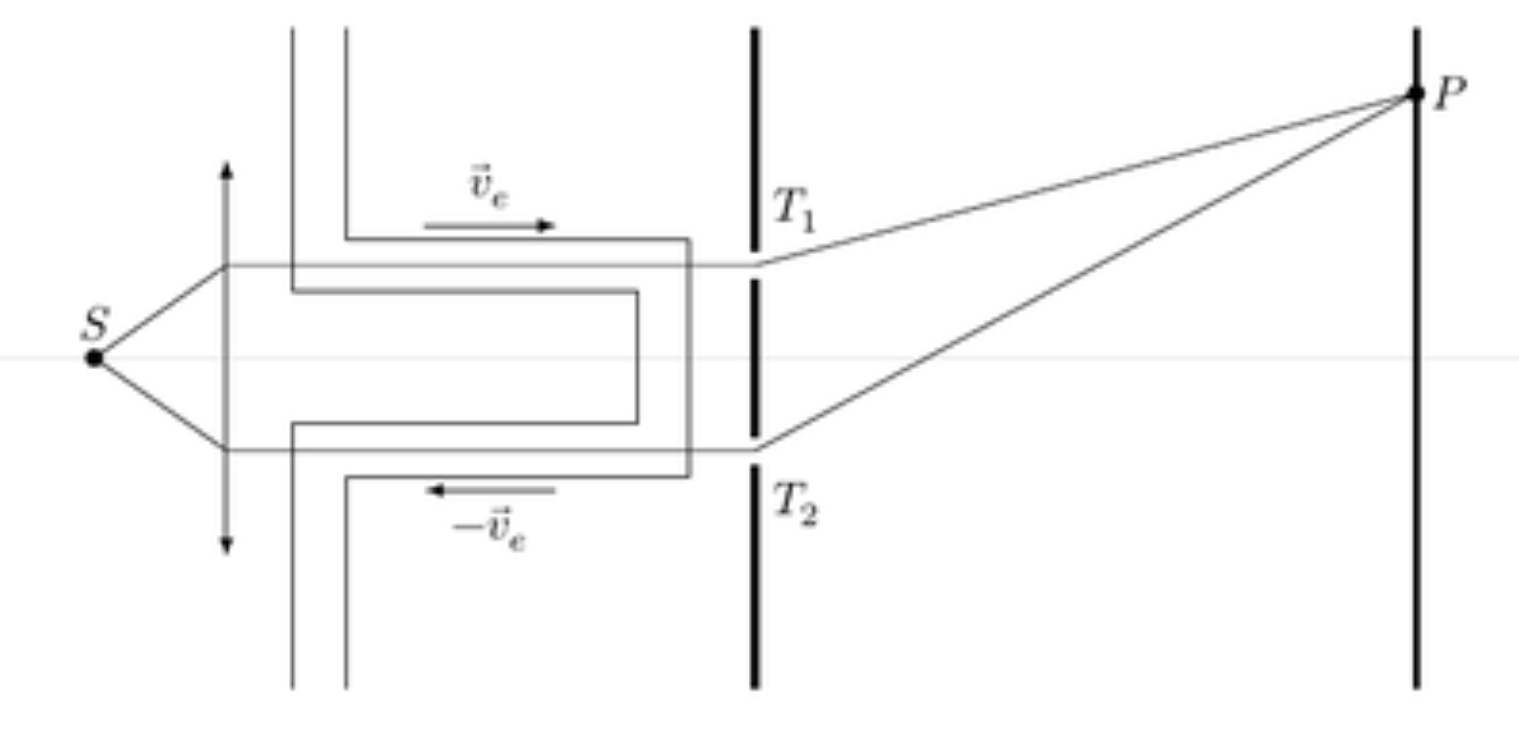
\includegraphics[width=.8\linewidth]{optique/interferences/expfizo.png}
    \caption{Schéma de l'expérience de Fizeau.}
\end{figure}

\begin{questions}
    \questioncours Différence de marche, ordre d'interférence
    \question Calculer l'ordre d'interférence au point $P$ en l'absence de courants d'eau ($v_e =0$).
    \uplevel{On suppose dans un premier temps que la vitesse de la lumière dans l'eau en mouvement à la vitesse $v_e$ vaut, dans le référentiel du laboratoire, $v = \frac{c_0}{n_e} + v_e$.}
    \question Justifier que cette hypothèse soit appelée `hypothèse galiléenne'.
    \question Calculer la variation de l'ordre d'interférence au point $P$ provoquée par l'établissement des courants d'eau.
    \question On observe un déplacement des franges de $\Delta x = 0.37 \pm 0.05$ mm, ceci est-il compatible avec l'hypothèse galiléenne ?
    \uplevel{On considère l'hypothèse relativiste suivante : la vitesse de la lumière dans l'eau en mouvement à la vitesse $v_e$ vaut, dans le référentiel du laboratoire, $v = \frac{c}{n_e} + v_e\qty(1-\frac1{n_e^2})$}
    \question Le déplacement des franges observé est-il en accord avec l'hypothèse relativiste ?
\end{questions}


\paragraph{Données :} Indice de l'eau au repos : $n_e = 1.337$

\end{exercise}

\section{Division d'amplitude}
\begin{exercise}{Mesure de l'indice de l'air}{1}{Spé}
{Interference, Michelson}{lelay}

Un interféromètre de Michelson est réglé de manière à observer des franges rectilignes en utilisant une source de lumière monochromatique à $\lambda_0 = 589$ nm. Sur l'une des voies, le faisceau traverse une cuve dont la longueur intérieure est $d = 10.0$ mm. Un détecteur mesure l'intensité de la lumière en un point fixe du champ d'interférences. Initialement, la cuve est vide et le détecteur est placé sur un maximum d'intensité.

On fait entrer de l'air dans la cuve, jusqu'à ce que la pression soit égale à la pression atmosphérique. On voit défiler alternativement 10 franges sombres et 9 franges lumineuses, et le détecteur indique finalement une intensité égale à la moitié de l'intensité maximale.

\begin{questions}
    \questioncours Interféromètre de Michelson
    \question Faire un schéma
    \question Déterminer l'indice de réfraction du gaz dans l'état final.
    \question Comment adapter cette expérience en utilisant des fentes d'Young à la place du Michelson ?
\end{questions}

\end{exercise}
\begin{exercise}{Modification des franges par effet Pockels}{1}{Spé}
{Interference, Michelson}{lelay}

Un interféromètre de Michelson est réglé en coin d'air d'angle $\alpha$ et éclairé sous incidence quasi-normale par une source de lumière monochromatique de longueur d'onde $\lambda_0 = 589$~nm. Sur l'une des voies de l'interféromètre, on dispose une lable de faible épaisseur $e$ et d'indice $n = 2.3$.

\begin{questions}
    \questioncours Décrire le montage utilisé à l'aide un schéma clair et en expliquant où sont localisées les interférences et comment faire pour les observer.
    \question Quel est l'effet de l'introduction de la lame sur le systèmes de franges ?
    \uplevel{En réalité, la lame est taillée dans un matériau dont l'indice peut varier lorsqu'il est soumis à un champ électrique $E$ intense (effet Pockels). La variation d'indice est de la forme $\Delta n = -\frac{n^3}{2}\ r\ E$, où $E$ est le champ électrique appliqué et $r$ un coefficient de réponse dépendant du matériau. 
    Le matériau utilisé est du nobiate de lithium (LiNbO$_3$) dont le coefficient de réponse est $r = 30$~pm/V.
    On impose à l'aide d'un générateur basse fréquence un champ électrique $E(t)$ oscillant triangulairement dans le temps avec un période $T$ et une amplitude $E_0 = 3$~kV/mm.}
    \question Comment choisir l'épaisseur de la lame pour que l'effet de la modulation soit observable ?
    \question Décrire ce que voit l'observateur.
\end{questions}

\end{exercise}


\begin{solution}

\begin{questions}
    \questioncours Coin d'air,. interf sur les miroirs, franges, rectilignes, une lentille fait l'image des miroirs sur un ecran.
    \question Diff de chemin optique $\delta = 2\ n_\text{air}\ \sin(\alpha)\approx 2\alpha$. Décalage de $\Delta x = -(n-1)e/\alpha$, l'interfrange $i = \lambda_0/2\alpha$ est inchangée.
    \uplevel{En réalité, la lame est taillée dans un matériau dont l'indice peut varier lorsqu'il est soumis à un champ électrique $E$ intense (effet Pockels). La variation d'indice est de la forme $\Delta n = -\frac{n^3}{2}\ r\ E$, où $E$ est le champ électrique appliqué et $r$ un coefficient de réponse dépendant du matériau. 
    Le matériau utilisé est du nobiate de lithium (LiNbO$_3$) dont le coefficient de réponse est $r = 30$~pm/V.
    On impose à l'aide d'un générateur basse fréquence un champ électrique $E(t)$ oscillant triangulairement dans le temps avec un période $T$ et une amplitude $E_0 = 3$~kV/mm.}
    \question On veut $\Delta\Delta x \geq i$ i.e. $e \geq \lambda_0/(2\Delta n)$. On trouve $e$ de l'ordre du mm.
    \question Si $T$ est court les franges sont brouillées. Si $T$ est long, on les voit se tranlater périodiquement
\end{questions}
\end{solution}

\begin{exercise}{Mesure d'ondes gravitationnelles}{2}{Spé}
{Interference, Michelson}{lelay}

Les détecteurs d’ondes gravitationnelles LIGO (USA) et VIRGO (Italie) sont des interféromètres à division d'amplitude. Leur structure est celle d’un interféromètre de Michelson dont les bras ont des longueurs effectives notées $L_1$ et $L_2$ de l'ordre de 300~km. . La source de lumière est un laser à $\lambda=1064$~nm d'intensité $I_0 = 125$~W. On note $A_1$ (resp $A_2$) l'amplitude de l'onde lumineuse passant par le bras 1 (resp. 2) au niveau du détecteur.
\begin{questions}
    \questioncours Expliquer le principe de fonctionnement d'un interféromètre de Michelson
    \question Dans chacun des bras de l'interféromètre on maintient un vide poussé ($10^{-6}$~Pa). Pourquoi à votre avis ?
    \question Exprimer la différence de phase $\Delta \phi$ entre $A_1$ et $A_2$ en fonction de $L_1$, $L_2$ et $\lambda$.
    \uplevel{Lorsqu’une onde gravitationnelle traverse l’interféromètre, elle distord l'espace ce qui allonge ou rétrécit légèrement les bras de l'interféromètre. On note donc $L_{1,2} = L^0_{1,2}+\delta L_{1,2}$ où $L_1^0$ et $L_2^0$ sont les longueurs au repos (en l'absence d'ondes gravitationnelles) et $\delta L_1$ et $\delta L_{2}$ reprśentent le changement de longueur des bras. On note $x_0 = L_1^0-L_2^0$ et $\delta x =\delta L_1-\delta L_2$.}
    \question La déformation relative $\delta x / L_1$ est de l'ordre de $10^{-21}$. Quel est l’ordre de grandeur de la variation de $\Delta \phi$ due à une onde gravitationnelle ? Peut–on observer un décalage de franges à l'oeil nu dans ces conditions ?
    \question L'intensité optique $I$ mesurée sur le détecteur est la moyenne temporelle du carré de l'onde lumineuse au niveau du détecteur $A=A_1+A_2$. Montrer que l'on peut exprimer $I$ sous la forme
    $$2 I_0\cos^2(\Delta\phi/2)$$
    \question En supposant $\delta x \ll \lambda$, montrer que l'on peut linéariser la variation d'intensité $\delta I$ sous la forme
    $$
    \delta I = -I_0\frac{4\pi \delta x}{\lambda}\sin(4\pi x_0 /\lambda)
    $$
    \question Pour quelles valeurs de $x$ cette variation intensité est-elle maximale ? En déduire comment est réglé l'interféromètre au repos.
    \question Quelle est l'intensité relative que le détecteur doit résoudre afin de détecter des ondes gravitationnelles ? Est-ce réaliste ?
    \question En réalité on place le détecteur sur une frange sombre. En déduire une nouvelle expression de la variation d'intensité.
    \question Comment faire pour maximiser la variation d'intensité mesurée ?
    
\end{questions}

\end{exercise}

\begin{solution}

\begin{questions}
    \questioncours Expliquer le fonctionnement d'un interféromètre de Michelson
    \question Variations faible pression indice = variation faible indice = cool. On prend donc $n=1$ dans la suite de l'exo   
    \question Trajet dans les deux bras, aller-retour donc $\delta = 2(L_1-L_2)/\lambda$. $\Delta \phi = 2\pi \delta = 4\pi(L_1-L_2)/\lambda$
    \uplevel{Lorsqu’une onde gravitationnelle traverse l’interféromètre, elle distord l'espace ce qui allonge ou rétrécit légèrement les bras de l'interféromètre. On note donc $L_{1,2} = L^0_{1,2}+\delta L_{1,2}$ où $L_1^0$ et $L_2^0$ sont les longueurs au repos (en l'absence d'ondes gravitationnelles) et $\delta L_1$ et $\delta L_{2}$ reprśentent le changement de longueur des bras. On note $x_0 = L_1^0-L_2^0$ et $\delta x =\delta L_1-\delta L_2$.}
    \question $\Delta \phi = 4\pi x_0 /\lambda + 4\pi \delta x/\lambda$. La contribution de l'onde gravitationnelle est le terme en $\delta x$, soit de l'ordre de $10\delta x/\lambda = 10^{-6}$ rad $\ll 1$. À l'oeil nu on peut résoudre le passage d'une frange brillante à une frange sombre, soit une différence de phase de $\pi$. On ne peut donc pas regarder ce décalage des franges directement : c'est un millionnième de ce qu'on mesure en TP.
    \question Interférences à 2 ondes (formule de Fresnel) : $I = A^2= I_0(1+\cos(\Delta \phi)) = I_0(1+ (2\cos^2(\Delta\phi/2)- 1)) = 2I_0\cos^2(\Delta\phi/2)$
    \question Il faut faire un DL à l'ordre 1, puisque $\qty(cos(x)^2)'= -\sin (2x)$, EN SUPPOSANT QUE $x_0$ EST NON NUL (modulo $\pi$)
    \begin{align*}
    \delta I &= -I_0\frac{4\pi \delta x}{\lambda}\sin(4\pi x_0 /\lambda)
    \end{align*}
    \question C'est maximal pour $\phi_0 = \frac{4\pi x_0}{\lambda} = \pi/2$ donc si les signaux sont au repos en quadrature de phase. C'est normal : faire un dessin de graphe de sinus, la plus grande variation est au moment où la dérivée est maximale, donc entre une frange sombre et une frange brillante.
    \question L'écart relatif entre l'intensité mesurée au repos et celle pendant une onde gravitationnelle est $\delta I/2I_0 \sim \delta x/\lambda = 10^{-7}$ : impossible de détecter 0.01 milliwatts de différence sur 100~W... Et en plus on crame le détecteur en lui envoyant 125 W dans la tronche.
    \question Sur une frange sombre, $\sin(4\pi x_0 /\lambda) = 0$ donc il faut pousser à l'ordre 2 le DL. On a
    \begin{align*}
    \delta I &=  -2I_0 \qty(\frac{2\pi \delta x}{\lambda})^2\cos(4\pi x_0 /\lambda) \\
    &=  - 8\pi^2 I_0 \qty(\frac{ \delta x}{\lambda})^2
    \end{align*}
    On est quadratique en $\frac{ \delta x}{\lambda}$ mais en même temps la variation relative d'intensité diverge donc c'est intéressant. Il me semble qu'en réalité c'est un compromis entre les deux qui est adopté.
    \question  Il faut un grand $I_0$ mais pas trop grand pour qu'il soit stable. Il faut aussi un faible lambda mais il faut tout de même un laser puissant... C'est difficile.
    
\end{questions}
\end{solution}

\section{Interférences à $N$ ondes}
% Niveau :      PCSI *
% Discipline :  Méca
% Mots clés :   Trajectoire particule chargée

\begin{exercise}{Iridescence d'une flaque d'huile}{3}{Spé}
{Optique ondulatoire, Fabry-Pérot,Réseau de Bragg}{bermu}

\begin{questions}
\questioncours Interférence à 2 ondes.

\begin{EnvUplevel}
\begin{figure}[H]
    \centering
    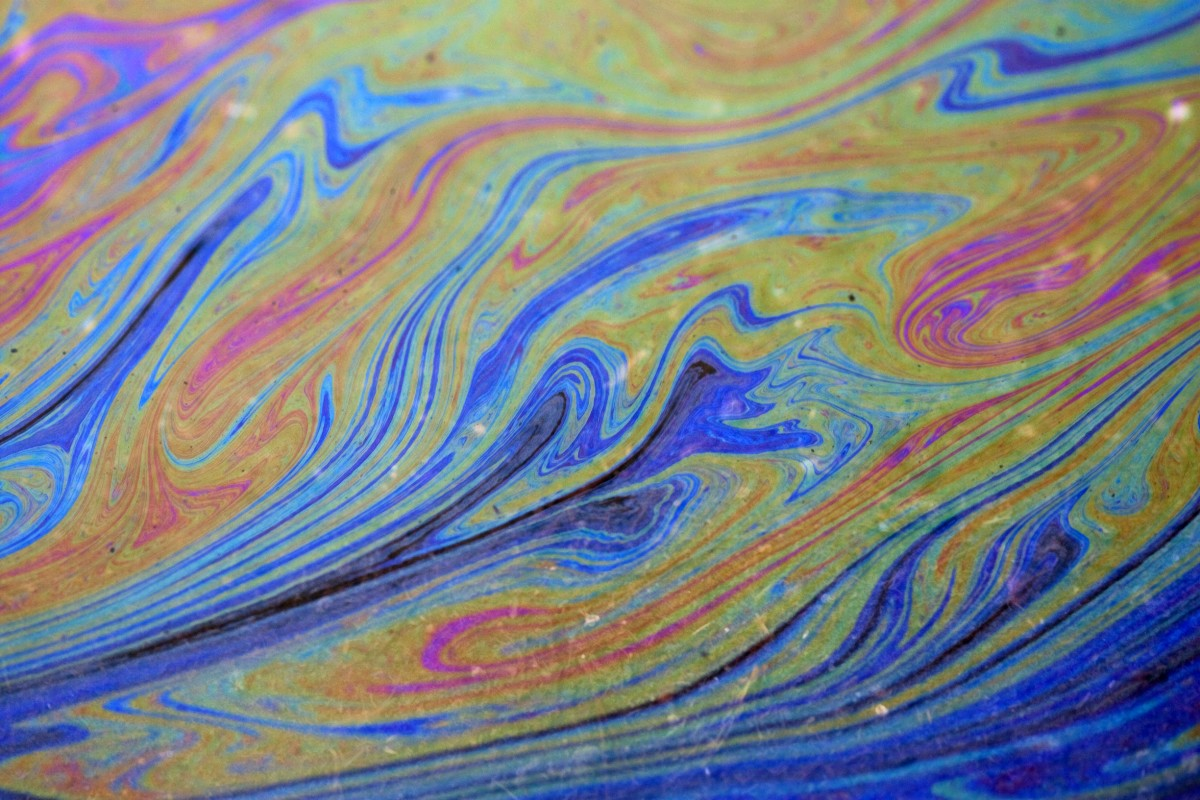
\includegraphics[width=.8\linewidth]{optique/interferences/iridescence.png}
    \caption{Irisations dans une flaque d'huile.}
    \label{fig:my_label}
\end{figure}

Nous allons à présent essayer de comprendre ce qui cause le phénomène d'iridescence lorsqu'il y a une tache d'huile sur une surface. On modélise pour cela la tache comme une couche d'huile d'épaisseur $e$ et d'indice $n = 1.5$ en surface du sol et surmontée d'air, d'indice 1. Un rayon lumineux de longueur d'onde $\lambda$ et d'intensité $I_0$ arrive sous incidence $\theta_1$.

Il est réfléchi/transmis de multiples fois. Le coefficient de réflexion en amplitude air/huile est noté $r$ et celui de transmission $t$. On considère que la réflexion est totale sur l'interface huile/sol.
\end{EnvUplevel}

\question Faire un schéma du modèle illustrant les réflexions multiples. Expliquer qualitativement le principe et où se formeront les interférences.

\question Quel est la différence de marche $\delta$ entre deux ondes réfléchies consécutives ? En quoi peut-on qualifier ce dispositif de réseau ?

\question Montrez que l'amplitude totale peut se mettre sous la forme suivante
$$A = A_0 \dfrac{r + (t^2-r^2) e^{i 2\pi\frac{\delta}{\lambda}}}{1 - r e^{i 2\pi\frac{\delta}{\lambda}}}.$$

\question En déduire la forme suivante pour l'amplitude
$$I = I_0\cal{F} \dfrac{\frac{(r+t^2-r^2)^2}{4r} + (t^2-r^2) \sin^2\qty(\pi\frac{\delta}{\lambda})}{1 + \cal{F} \sin^2\qty(\pi\frac{\delta}{\lambda})},$$
avec $\cal{F}$, la finesse de l'interféromètre dont on pourra donner l'expression et une interprétation physique.

\uplevel{Pour une onde polarisée correctement$^\dagger$, les coefficients de réflexion en amplitude sont
$$r = \dfrac{\cos\theta_1 - n \cos\theta_2}{ \cos\theta_1 + n \cos\theta_2}, \qquad t = 1 + r,$$
avec $\theta_2$ l'angle de réfraction dans l'huile.}

\question Comment ce simplifie cette expression sous incidence quasi-normale ? Tracer le profil $I(x = \delta/\lambda)$. Interpréter ces résultats au vue de la figure ci-dessus.
\end{questions}

$^\dagger$ {\small Polarisation dite transverse électronique ou s.}
\end{exercise} 

\begin{solution}


\begin{questions}
\questioncours Interférence à 2 ondes.

\question À l'infini : il faut être loin (devant $e$), ou mettre une lentille.

\question $\delta = 2ne \cos\theta_1$, au moins aux petits angles...

\question On somme, bien faire attention à ne pas faire la récurrence trop vite

\question  $\cal{F} = \frac{4r}{1-r^2}$ (comme pour un FP normal), rend compte de la selectivite du dispositif

\uplevel{Pour une onde polarisée correctement$^\dagger$, les coefficients de réflexion en amplitude sont
$$r = \dfrac{\cos\theta_1 - n \cos\theta_2}{ \cos\theta_1 + n \cos\theta_2}, \qquad t = 1 + r,$$
et le coefficient en intensité $R = \abs{r}^2$.}

\question Inicidence quasi normale: $\theta_1\approx\theta_2\approx 0$ i.e. $r\approx \frac{1-n}{1+n}$. La fonction d'airy a des pics très piqués : Si on change nu peu de lambda, on change un peu où on a des interf constructives. Faire dire que l'epaisseur de la lame d'huile doit etre d'ordre de $\lambda$ sinon ça ne marche pas.
\end{questions}

\end{solution}
\begin{exercise}{Couleur d'une émulsion ferrofluide}{1}{Spé}
{Interference, Fabry-Pérot}{lelay}

Une émulsion ferrofluide est composée de gouttelettes de ferrofluide de rayon négligeable, placées dans l'eau d'indice $n = 1.33$. Lorsqu'on soumet le ferrofluide à un champ magnétique, les goutelettes s'organisent en chaînes, la distance entre deux gouttelettes est une constante $d = 220$~nm et toutes les chaînes sont parallèles à une direction $Ox$. On éclaire l'émulsion avec de la lumière blanche se propageant dans la direction $Ox$ et on observe la lumière récupérée dans la direction $-Ox$, due à la diffusion de la lumière par les goutelettes, c'est-à-dire à l'absorption partielle de l'onde incidente et à la réémission d'une onde en phase.

On constante que la lumière est nettement colorée. 

\begin{questions}
    \question Interpréter ces observations
    \question Quelle est la couleur de la solution ?
    \question Lorsqu'on augmente la température, $d$ augmente. Comment alors varie la couleur de la solution ?
\end{questions}

\end{exercise}


\begin{solution}

\begin{questions}
    \question Interf constructive nombreuse à la fabry perot
    \question $\delta = 2nd$, constructif si $\delta = p\lambda_0$. $\lambda_0 = 2nd = 585$~nm, jaune-orangé.
    \question Vers le rouge.
\end{questions}
\end{solution}
\begin{exercise}{Système optomécanique}{3}{Spé}
{Interférences, pression de radiation, Fabry-Pérot}{lelay}

On considère le système optomécanique réprésenté ci-dessous : la lumière est introduite dans le système par la gauche dans une cavité de section transverse $S$ formée par deux miroirs. Le miroir de gauche est immobile et parfaitement réfléchissant, le miroir de droite est mobile, a un coefficient de réflexion $r$ très proche de 1, possède une masse $m$ très faible et est relié au fond de la cavité par un ressort de raideur $k$.

\begin{center}
    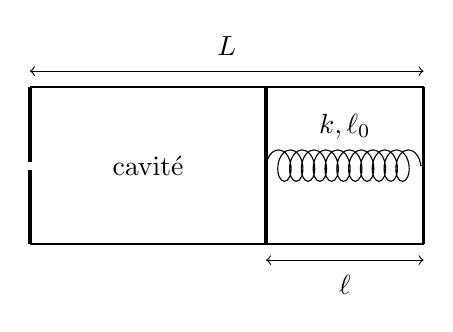
\begin{tikzpicture}
    \draw[<->] (-1,1.2) -- (4, 1.2);
    \draw (1.5,1.2) node[above=2pt] {$L$};
    
    % \fill[black!5]  (0,-1) rectangle (2,1);
    \draw[ultra thick] (-1,-1) -- (-1, -0.05);
    \draw[ultra thick] (-1,0.05) -- (-1, 1);
    \draw[thick] (-1,-1) -- (4,-1);
    \draw[thick] (-1, 1) -- (4, 1);
    \draw[ultra thick] (2,-1) -- (2, 1);
    \draw (0.5,0) node[anchor=center] {cavité};
    
    \draw[decoration={aspect=0.6, segment length=1.5mm, amplitude=2mm,coil},decorate] (2,0) -- (4,0);
    \draw[thick] (4,-1) -- (4, 1);
    \draw (3,0) node[above=6pt] {$k, \ell_0$};

    \draw[<->] (2,-1.2) -- (4, -1.2);
    \draw (3,-1.2) node[below=2pt] {$\ell$};
    
    \end{tikzpicture}
\end{center}

\begin{questions}
    \questioncours Phénomène d'interférences
    \question Calculer $I$, l'intensité lumineuse sur le miroir.
    \uplevel{La lumière est composée de photons, d'énergie $h\nu$ et de quantité de mouvement $h/\lambda$ (relation de De Broglie). On note $n$ la densité volumique de photons en un point.}
    \question En assimilant l'énergie du champ électromagnétique à celle des photons, donner un lien entre $n$ et $I$.
    \question En déduire, à l'aide d'un bilan de quantité de mouvement sur un temps $\dd{t}$, la force de pression de radiation qu'une onde lumineuse d'intensité $I$ exerce lorsqu'elle est réfléchie sur un miroir perpendiculaire à sa direction de propagation
    \question Donner les positions d'équilibre du miroir mobile et de leur stabilité.
\end{questions}
\end{exercise}

\begin{solution}

\begin{questions}
    \questioncours Phénomène d'interférences
    \question C'est un fabry-Pérot. Entre deux aller-retours, la différence de marche est $\delta = 2(L-\ell)$ d'où un déphasage $\Phi = 2\pi \delta/\lambda = 4\pi(L-\ell)/\lambda$ et l'amplitude est divisée par $r$, on trouve 
    \begin{align}
        A = A_0 + r A_o e^{i\Phi} + \cdots= \frac{A_0}{1 - re^{i\Phi}}
    \end{align}
    d'où l'intensité 
    \begin{align}
        I &= |A|^2 = \frac{I_0}{1 + r^2 - 2r\cos\Phi} \\
        &= \frac{I_0}{(1-r)^2} \frac{1}{1 + \cal{F}\sin^2(\Phi/2)}
    \end{align}
    sous la forme de la fonction d'Airy, avec la finesse standard $\cal{F} = 4r/(1-r)^2$.
    
    FAIRE TRACER LA COURBE AUX ETUDIANTS

    Puisque $r$ est proche de 1, on prendra la finesse très grande et donc les franes brillantes sont très piquées.
    \uplevel{La lumière est composée de photons, d'énergie $h\nu$ et de quantité de mouvement $h/\lambda$ (relation de De Broglie). On note $n$ la densité volumique de photons en un point.}
    \question Densité d'energie EM $\frac12 \epsilon_0 E^2$, intensité lumineuse $I = E^2$, densité d'énergie photonique $n h \nu$ d'où $n h \nu = \frac12 \epsilon_0 I$ et donc $n =\epsilon_0 I/(2 h \nu)$
    \question Pendant $\dd{t}$ le miroir réfléchit $n (c\dd{t}) S$ photons de qté de mvt $h/\lambda$ d'où $\dd{p} = n c S \dd{t} \cdot 2 \cdot h/\lambda = 2 n h \nu S \dd{t} =\epsilon_0 I S \dd{t}$ et donc la force de pression de radiation $P = \epsilon_0 I$.
    \question Résolution graphique : Tracer $P(\ell)$ (successions de pics fins) et la force du ressort $F(\ell)$ (droite décroissante), voir où sont les intersections. Discuter le cas d'une raideur très grande, très petite. À chaque intersection de la droite avec un pic il y a une position stable et une instable (je crois). On peut calculer la freq des petites oscillations en faisant un DL ? Discuter en tout cas les pertes, qui n'ont pas été abordées ici.
\end{questions}
\end{solution}


% Niveau :      PCSI *
% Discipline :  Méca
% Mots clés :   Trajectoire particule chargée

\begin{exercise}{Minimum de déviation}{1}{Spé}
{Optique ondulatoire, Réseau}{bermu}

On considère une onde plane progressive harmonique, de longueur d'onde $\lambda$ en incidence $\theta$ sur un réseau de diffraction plan en transmission de pas $a = \SI{100}{µm}$.

\begin{questions}
\questioncours Donner la relation fondamentale des réseaux.

\uplevel{On appelle déviation l'angle $D$ entre les directions incidente et diffractée.}

\question Calculer le minimum de déviation du réseau.

\end{questions}
\end{exercise} 

\begin{solution}


\begin{questions}
\questioncours $\sin\theta' - \sin\theta = p\lambda/a$

\question $D = \theta' - \theta$. Le minimum est donc pour $\dv{\theta' - \theta}{\theta} = 0$ donc $\dv{\theta'}{\theta} = 1$.

Or $\sin\theta' - \sin\theta = p\lambda/a$, donc par dérivation $\cos\theta' = \cos\theta$. Donc plusieurs cas

\begin{itemize}
    \item $\theta = \theta'$ : $D_m = 2\theta$ (réseaux en transmission)
    \item $\theta = -\theta'$ : $D_m = 0$ (réseaux en réflexion)
\end{itemize}
\end{questions}

\end{solution}



\begin{exercise}{Réseau blazé}{2}{Spé}
{Optique ondulatoire, Réseau}{bermu}

On considère un réseau de diffraction plan en réflexion de pas $a$ éclairé en incidence $i$ par un faisceau parallèle de lumière monochromatique de longueur d'onde $\lambda = 530$ nm.

\begin{questions}

\questioncours Donner la formule des réseaux.

\question Quelle est la différence de marche entre deux rayons frappant deux motifs successifs sous la même incidence $i$ et émergeant sous l’angle $i’$ ? \`A quelle condition observe-t-on un maximum de l’éclairement du aux interférences ? Comment évolue l'intensité de ces maxima en fonction de l'ordre ?

\uplevel{Un réseau blazé est obtenu en traçant sur une surface métallique des dents de scie dont la coupe
est représentée ci-contre. Les bandes utiles réfléchissantes ont pour largeur $b$, sont inclinées d'un angle $\alpha$ et constituent un réseau de $N$ bandes de pas $a$.
\begin{figure}[H]
    \centering
    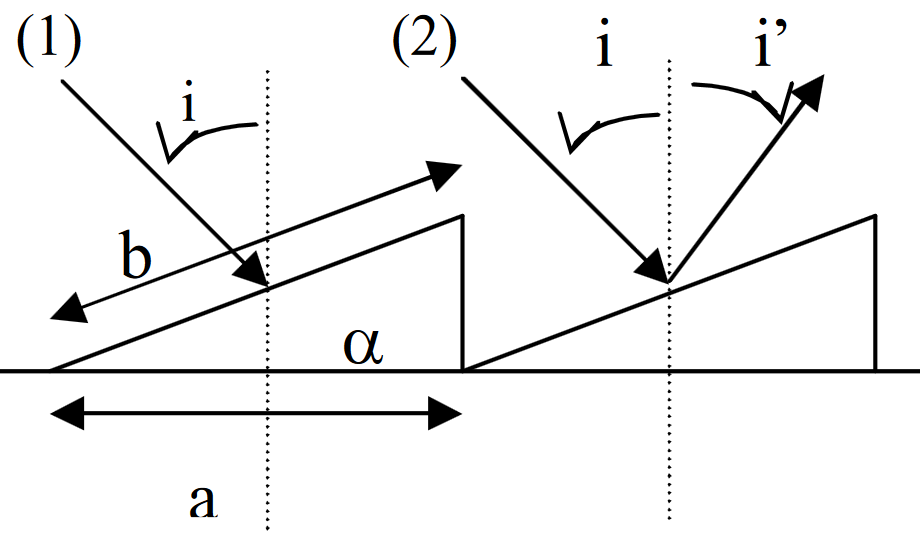
\includegraphics[width=0.4\linewidth]{optique/interferences/reseau-blaze.png}
    \caption{Schéma de principe d'un réseau blasé.}
\end{figure}

On observe les ondes diffractées dans la direction $i'$ à l'infini.
}

\question D'après ce que vous savez sur l'optique géométrique, en quel angle $i_0'$ se trouvera le maximum de diffraction ?

\question On souhaite faire coïncider ce maximum de diffraction avec le maximum d'interférence de l'ordre $p$. Quelle relation doit alors vérifier l'angle de blaze $\alpha_p$ ? En quoi cela est intéressant contrairement à un réseau plan simple ?

\question Le réseau utilisé comporte 200 motifs/mm. Il est utilisé en autocollimation ($i=0$) et concentre l’énergie
dans l’ordre 4. Donner l'angle de blaze de ce réseau. Comment pourriez-vous distinguer expérimentalement ce réseau d’un réseau plan ?

\end{questions}
\end{exercise} 

\begin{solution}


\begin{questions}
\questioncours $\sin i' - \sin i = p\lambda/a$

\question $\delta = a(\sin i' - \sin i) = -p\lambda$.

L'intensité des maxima diminue dramatiquement avec l'ordre. Presque tout est concentré dans l'ordre 0, ce qui est bête.

\question L'angle max est l'angle de réflexion des lois de Descartes. $\theta = \theta'$ (par rapport à la normale au dioptre) soit $i - \alpha = i' + \alpha$. $i = i' + 2\alpha$.

\question Pour coïncider avec $i'_p$ tel que $a(\sin i'_p - \sin i) = -p\lambda$, avec également $i'_p = i - 2\alpha$, on veut $$\sin (2\alpha - i) + \sin i = p\lambda/a.$$

La lumière est maintenant dans l'ordre $p$ ce qui est quand même plus intéressant.

\question On veut donc $\sin (2\alpha) = 4\lambda/a$ (...)

On le distingue par le fait que l'ordre 0 est peu lumineux i.e. on ne voit ce qu'il y a en face pas au travers.
\end{questions}

\end{solution}





% Niveau :      PCSI *
% Discipline :  Méca
% Mots clés :   Trajectoire particule chargée

\begin{exercise}{Pouvoir de résolution du réseau}{3}{Spé}
{Optique ondulatoire, Réseau}{bermu}

On considère une onde plane progressive harmonique, de longueur d'onde $\lambda$ en incidence normale sur un réseau de diffraction plan en transmission de pas $a = \SI{100}{µm}$.

\begin{questions}
\questioncours Décrire le principe du réseau.

\question Établir la différence de marche entre deux ondes issues de deux fentes consécutives du réseau dans la direction $\theta$. Pour quelles directions aura-t-on des interférences constructives ?

\question Calculer amplitude complexe de l'onde lumineuse à l'infini dans la direction $\theta$. On notera $N$ le nombre de fentes (uniformément) éclairées par l'onde incidente.

\question Calculer l'intensité lumineuse de l'onde à l'infini $I(\theta)$. Quelles sont les maxima de l'intensité ? Donner la largeur angulaire $\delta\theta$ des pics d'intensité maximale.

\uplevel{On considère maintenant le réseau éclairé en lumière polychromatique. On appelle pouvoir de résolution la quantité $P = \dfrac{\lambda_m}{\delta\lambda_m}$, ou $\delta \lambda_m$ est la différence minimale entre deux longueurs d'onde que le système peut séparer, et $\lambda_m$ leur moyenne.}

\question Rappeler le critère de Rayleigh sur la résolution de deux pics $\theta_1$ et $\theta_2$ dont la largeur angulaire est $\delta\theta$.

\question \`A l'aide des questions précédentes, établir le pouvoir de résolution de ce réseau.

\end{questions}
\end{exercise} 

\begin{solution}

\begin{questions}
\questioncours Des trous de taille $a$...

\question Faire un beau schéma. $\delta = a\sin\theta$. On a donc interférence pour $p = \delta/\lambda$ entier soit
$$\sin\theta_p = p\lambda/a.$$

\question $s(\theta) = \sum_{k=0}^{N} s_0 e^{i2\pi k \delta/\lambda} = s_0 \dfrac{e^{i2\pi N \delta/\lambda} - 1}{e^{i2\pi \delta/\lambda} - 1} = s_0 e^{i2\pi (N-1) \delta / \lambda} \dfrac{\sin(\frac{N\pi\delta}{\lambda})}{\sin(\frac{\pi\delta}{\lambda})}.$

\question $I(\theta) = I_0 \dfrac{\sin^2\qty(\frac{N\pi\delta}{\lambda})}{\sin^2\qty(\frac{\pi\delta}{\lambda})}.$
Maximum en $\theta = \theta_p$. Autour $\theta = \theta_p \pm \delta\theta/2$, on annule le numérateur si $N\pi\delta/\lambda = (p\pm1)\pi$, soit $\sin(\theta_p \pm \delta\theta/2) = \frac{p\pm1}{a N}$ soit
$$\delta\theta = \dfrac{2\lambda}{N a \cos\theta_p}$$

\question Critère de Rayleigh : $\theta_1 - \theta_2 > \delta\theta/2$.

\question Ainsi, on doit avoir : $\theta(\lambda_m + \delta\lambda/2) - \theta(\lambda_m - \delta\lambda/2) > \dfrac{2\lambda}{N a \cos\theta_p}$ et comme $\sin\theta_p = p\lambda/a$ :
$$\sin\theta(\lambda_m + \delta\lambda/2) - \sin\theta(\lambda_m - \delta\lambda/2) = 2 p\delta\lambda/a \cos\theta_p$$
enfin
$$\delta\lambda = \lambda/ pN \qqtext{soit} P = pN.$$


\end{questions}

\end{solution}


\section{Diffraction et filtrage optique}

\section{Laser}